\documentclass[a4paper,12pt]{article}
\usepackage{geometry}
\usepackage{color}
\usepackage{graphicx}
\usepackage{amsmath}
\usepackage{multirow}
\usepackage{float}
\usepackage{forest, array}
\usepackage{listings}


\geometry{left=3.18cm, right=3.18cm, top=2.54cm, bottom=2.54cm}
\begin{document}

\textbf{CS-GY 6643 Computer Vision Spring 2021}

\textbf{Instructor: Prof. James Fishbaugh}

\textbf{Final Project Proposal}

\textbf{Team Members: Zhe Luan(zl3368) Tianyi Zhao(tz1330)}

\vskip\baselineskip
\textbf{Title: Chess Image Recognition Using Traditional Computer Vision Techniques and Neural Networks}

\vskip\baselineskip

\noindent \textbf{1. Introduction}



Tencent's Fox Go, a popular go chess game platform which has one of the most powerful go Ai FineArt, has recently released a mobile application which can recognize go chessboard and go pieces. It can output a 2D image of the go-chessboard and help judge the game. Inspired by this application, we want to implement a chess board and chess pieces recognition application. 



\vskip\baselineskip
\noindent \textbf{2. Objectives}

Figure 1 is the original go chessboard and chess pieces image. Figure 2 is the recognized image by Tencent's fox go mobile application (https://apps.apple.com/cn/app/id1022649876). We want to do the similar transformation from a chessboard in real world to a digital image, as Figure 3 shows.

\begin{figure}[H]
	\centering
	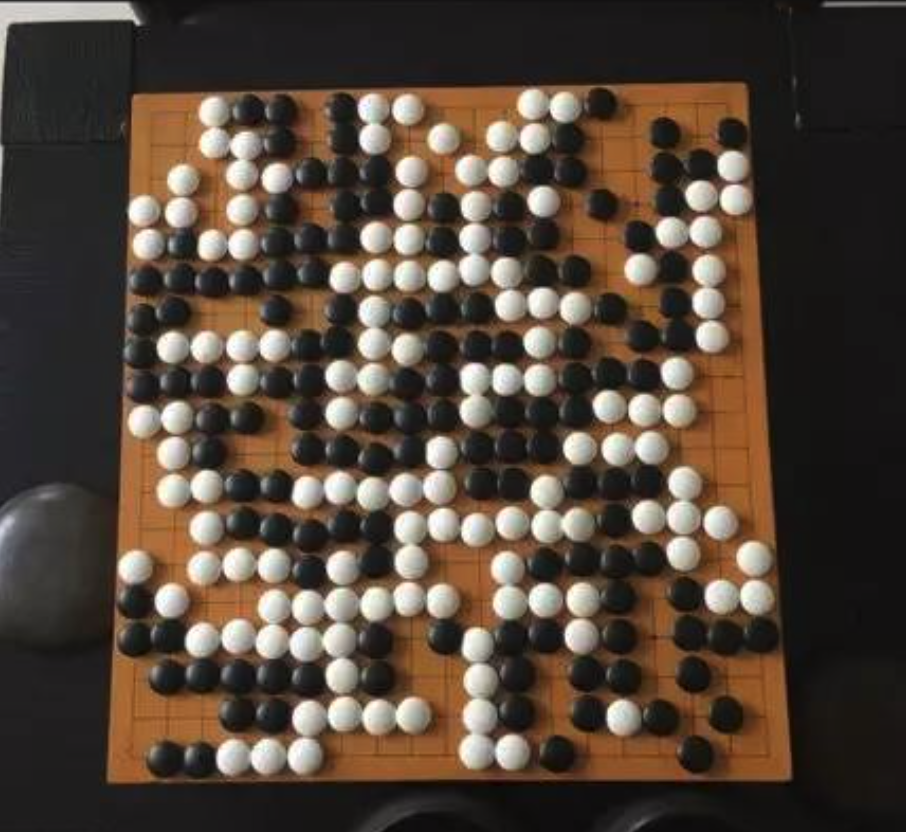
\includegraphics[scale=0.2]{1.png}
	\caption{Original go chessboard.}
\end{figure}

\begin{figure}[H]
	\centering
	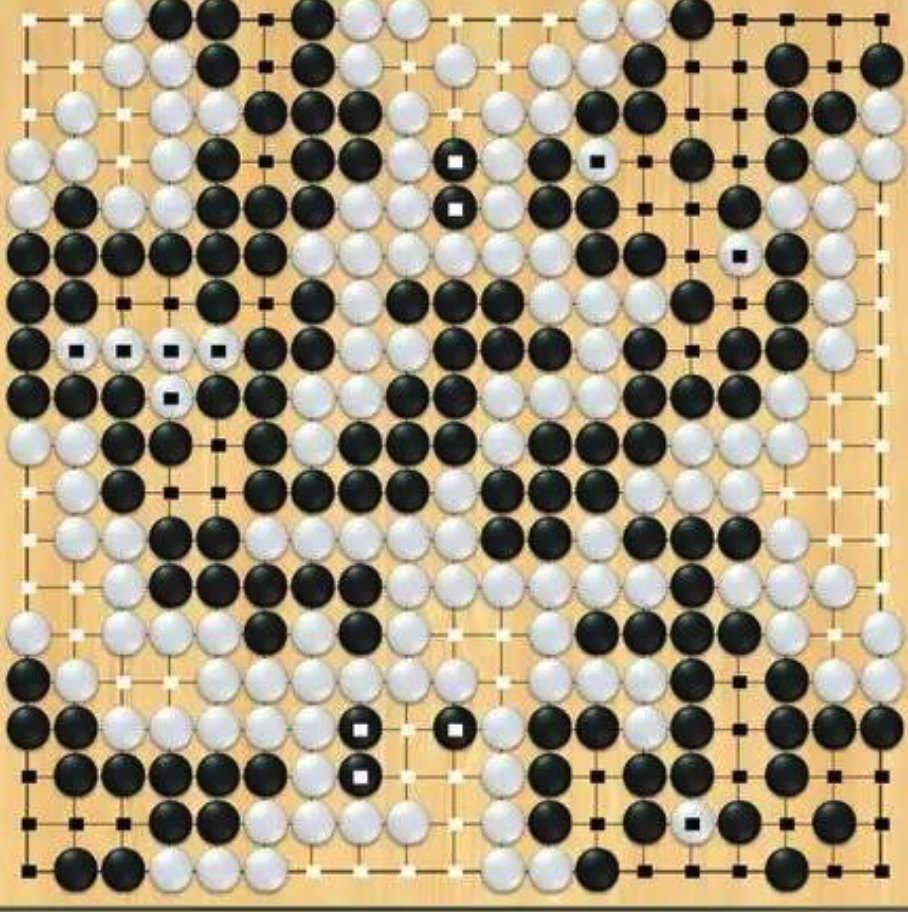
\includegraphics[scale=0.2]{2.png}
	\caption{2D output image recognized by fox go mobile application.}
\end{figure}

\begin{figure}[H]
	\centering
	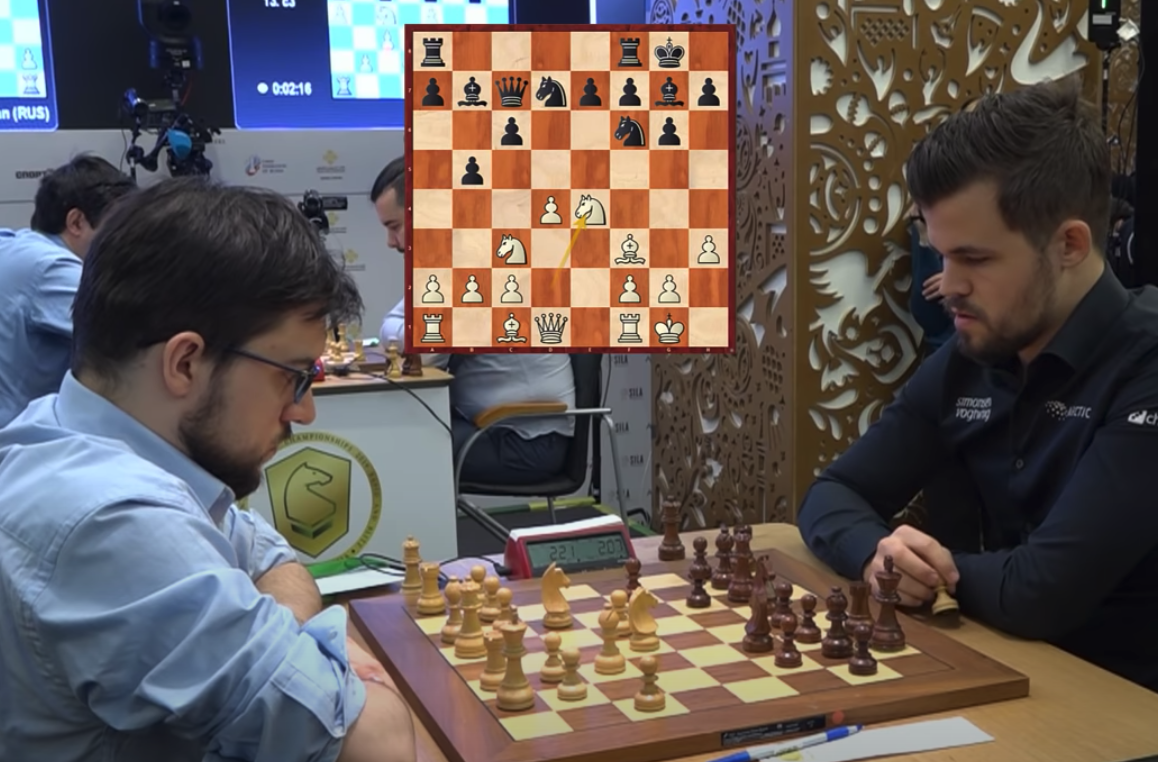
\includegraphics[scale=0.2]{3.png}
	\caption{Recognizing a real world chessboard. MVL vs Carlsen World Championship 2020.}
\end{figure}

\vskip\baselineskip
\noindent \textbf{3. Approaches}

We can break this project to two parts, chessboard recognition and chess pieces recognition and positioning. The first part should be straightforward in computer vision. We can use traditional CV techniques such as edge detection and Hough transformation.

Different from go pieces, chess pieces recognition is more complicated since there are 6 types of chess pieces of both black and white pieces, so we intend to use some deep learning techniques such as CNN to do this part.

\vskip\baselineskip
\noindent \textbf{4. Data}

We have found some online open source chessboard and chess pieces image data. We will use them to train and verify our model. We will also take photos of our own chess and use these photos to test our work.

\begin{itemize}
	\item https://www.dropbox.com/sh/8s4tvir5zbotseq/AACAQypmuFb6j-Yww9x9Q6Gta?dl=0
	\item https://public.roboflow.com/object-detection/chess-full
\end{itemize}

\vskip\baselineskip
\noindent \textbf{5. Reference}

\noindent 1. ChessVision: Chess Board and Piece Recognition. Jialin Ding. Stanford University. \\
https://web.stanford.edu/class/cs231a/prev\_projects\_2016/CS\_231A\_Final\_Report.pdf

\vskip\baselineskip
\noindent 2. Chess Piece Recognition Using Oriented Chamfer Matching with a Comparison
to CNN. Youye Xie, Gongguo Tang, William Hoff. Colorado School of Mines, Golden, Colorado USA. \\
https://par.nsf.gov/servlets/purl/10099572
\end{document}